\clearpage{\pagestyle{empty}\cleardoublepage}
\chapter{Sviluppo dell'elaborato di progetto}

In questo progetto verrà descritto il progetto sviluppato, in particolare l'architettura generale del sistema,
la descrizione dei singoli componenti e l'applicazione front-end.

\section{Architettura generale del sistema}

In questa sezione verrà descritta l'architettura generale del sistema, analizzando i componenti principali,
le loro interazioni e le scelte progettuali adottate.

\subsection{Architettura a microservizi}

Il progetto AirQualityInsight è stato realizzato utilizzando un'insieme di microservizi.

I microservizi rappresentano un approccio architetturale per lo sviluppo di applicazioni software che prevede
la scomposizione di un sistema monolitico, dove tutti i processi sono interdipendenti e funzionano come un singolo
servizio, in un insieme di servizi indipendenti, ognuno dei quali implementa una specifica funzionalità
di business \cite{newman2015building}. Ogni microservizio viene eseguito nel proprio processo e comunica attraverso
\acrshort{api} \acrshort{rest} (\acrlong{rest}), event streaming e broker di messaggistica asincrona
\cite{fowler2014microservices}.

Le caratteristiche distintive di questa architettura includono l'autonomia di deployment, la responsabilità
su specifici domini di business, la gestione decentralizzata dei dati e la possibilità di utilizzare
tecnologie eterogenee per diversi servizi. Utilizzare i microservizi piuttosto che un sistema monolitico
semplifica l'aggiornamento del codice, permette di implementare nuove funzionalità senza modificare
l'intera architettura applicativa, aumenta il grado di libertà nella scelta sulle tecnologie e linguaggi
di programmazione da adottare, che possono così essere differenti per ciascun componente,
favorisce la scalabilità orizzontale e consente di dimensionare indipendentemente ogni servizio
in base alle specifiche esigenze di carico \cite{dragoni2017microservices}, eliminando gli sprechi e riducendo i costi
derivanti dalla necessità di scalare l'intera applicazione quando solo una specifica funzione
richiede risorse aggiuntive.

Tuttavia, l'adozione dei microservizi introduce anche sfide significative, tra cui la complessità nella gestione
della comunicazione inter-servizio, la necessità di implementare pattern di resilienza e la gestione della consistenza
dei dati in un ambiente distribuito \cite{richardson2018microservices}. La governance e il monitoraggio
di sistemi distribuiti richiedono inoltre strumenti e pratiche specifiche
per garantire osservabilità e debugging efficaci \cite{wolff2016microservices}.

In conclusione, questo approccio offre vantaggi nella progettazione di sistemi complessi, rendendo più chiara
la suddivisione dei vari aspetti del dominio applicativo, e nella realizzazione degli stessi,
facilitando la resilienza del sistema.

\subsection{Architettura del sistema}

L'architettura del sistema AirQualityInsight si basa su 5 componenti principali, come illustrato
in figura \ref{fig:architecture}: i sensori atti a realizzare misurazioni simulate, il broker di messaggistica,
il server per la fruizione degli stessi, la dashboard front-end ed infine il database non relazionale.

\begin{figure}[H]
  \centering
  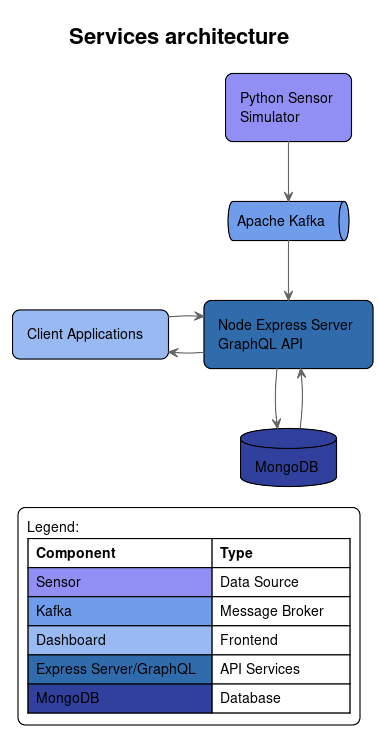
\includegraphics[width=0.5\textwidth]{architecture.png}
  \caption{Architettura generale del sistema}
  \label{fig:architecture}
\end{figure}

Di seguito vengono esplicitate le varie responsabilità per ognuno dei servizi precedentemente elencati.

\begin{itemize}
  \item Sensor service: questo servizio simula l'esercizio di un insieme di sensori, i quali registrano,
        con cadenza regolare, le misurazioni della qualità dell'aria. Ogni sensore è provvisto di un id univoco,
        un nome, una posizione geografica (le coordinate della sua collocazione) ed un indirizzo IP.
        Tali misurazioni vengono inviate al broker dei messaggi in modo che vengano poi trasmesse ai servizi in ascolto.
  \item Broker service: questo servizio dispone di un canale di comunicazione logico (topic)
        dove vengono pubblicate e consumate le informazioni. Nel canale vengono accodate le misurazioni
        ottenute dai sensori, le quali sono poi consumate dal servizio del server \acrshort{api},
        per la loro gestione ed erogazione.
  \item \acrshort{api} Server service: questo servizio consuma dal broker le misurazioni, le salva
        sul database non relazione e le rende disponibili attraverso \acrshort{api}.
  \item Dashboard service: questo servizio fornisce un'interfaccia grafica tramite cui è possibile consultare
        la mappa interattiva, aggiornata in tempo reale con i dati forniti dal server \acrshort{api}, e le relative
        tabelle.
  \item Database service: questo servizio si occupa di salvare in modo persistente le misurazioni
        registrate dai sensori, permettendo future interrogazioni sui dati storici.
\end{itemize}

\section{Sensor service}

In questa sezione verrà descritto il servizio che simula il sensore e la relativa generazione di misurazioni fittizie
sulla qualità dell'aria.

\subsection{Modello sensore}

Il sensore è dotato di un insieme di proprietà specifiche che ne determinano il funzionamento.
Queste proprietà sono:

\begin{itemize}
  \item Id (\texttt{sensor\_id}): stringa, identificatore univoco del sensore.
  \item Nome (\texttt{name}): stringa, nome del sensore.
  \item Posizione (\texttt{location}): oggetto, posizione in cui è collocato il sensore.
        Si tratta di un oggetto composto dal tipo (in questo caso \texttt{Point}) e dalle coordinate,
        longitudine e latitudine, ambo valori numerici a virgola mobile (\texttt{double}).
  \item IP (\texttt{ip}): stringa, indirizzo ip del sensore.
  \item Attivo (\texttt{active}): booleano, indica se il sensore è attivo (\texttt{true})
        oppure no (\texttt{false}).
  \item Ultima misurazione (\texttt{last\_seen}): data, ultima volta che il sensore ha registrato una misurazione.
        \label{lst:sensors-properties}
\end{itemize}

\subsection{Distribuzione sensori}

La scelta dei sensori è stata fatta relativamente ai punti di maggiore traffico, quali le intersezioni stradali
fra le arterie principali e le strade secondarie. Bologna presenta una moltitudine di semafori, luogo dove macchine
ferme in attesa tendono a creare punti di maggiore concentrazione di inquinanti. Come anticipato precedentemente
con la query \ref{lst:overpass-query}, sono stati estrapolati tutti i punti che rappresentano un'intersezione
stradale di questo tipo. Data l'elevata densità di posizioni rilevate, è stata applicata una selezione sistematica
per mantenere un singolo punto per ogni intervallo spaziale regolare.
Questa selezione ha permesso anche di gestire le situazioni di affollamento, tipiche di rotonde,
nelle quali ogni svincolo è rappresentato come incrocio, e di centri abitati, nei quali la concentrazione
di queste intersezioni risulta più elevato.

Nelle immagini \ref{fig:sensors-before} e \ref{fig:sensors-after} viene mostrato come, partendo da un dataset
consistente di punti, siano stati poi filtrati secondo i criteri precedentemente esposti.
È stata implementata una griglia di campionamento con spaziatura di 250 metri, parametro calibrato
sperimentalmente per ottenere una densità ottimale di punti. Per fare ciò è stata realizzata una pagina dedicata
allo scopo, essendo un processo che può essere riprodotto cambiando la distanza fra i punti tramite input numerico.

\begin{figure}[H]
  \centering

  \begin{subfigure}{\textwidth}
    \centering
    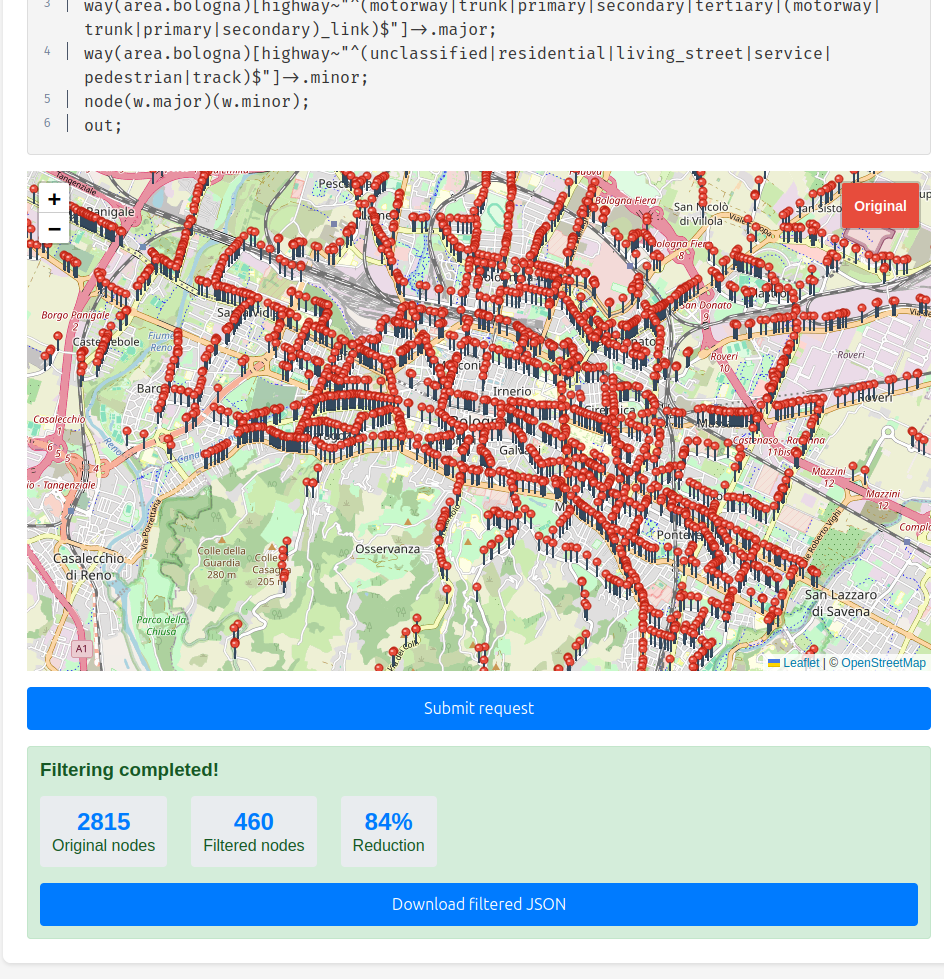
\includegraphics[width=0.75\textwidth]{sensors/00_before.png}
    \caption{Risultato originale della query}
    \label{fig:sensors-before}
  \end{subfigure}

  \hfill
  \begin{subfigure}{\textwidth}
    \centering
    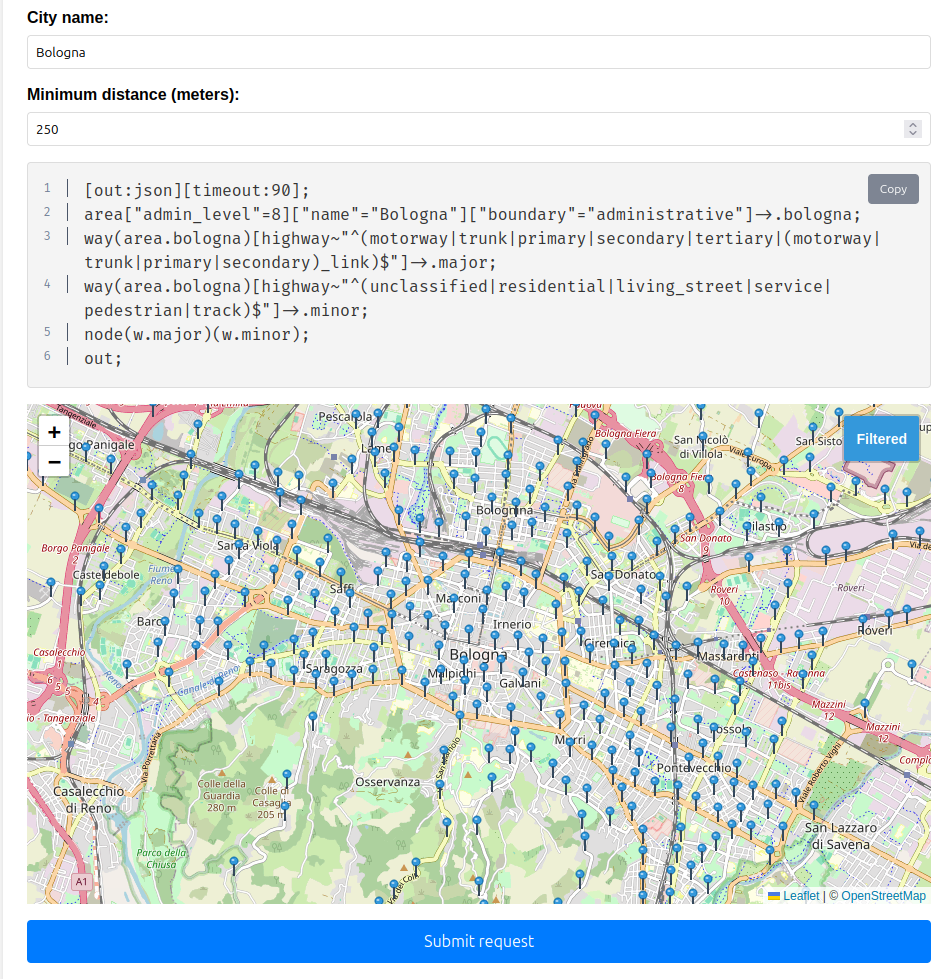
\includegraphics[width=0.75\textwidth]{sensors/01_after.png}
    \caption{Punti filtrati finali}
    \label{fig:sensors-after}
  \end{subfigure}

  \caption{Acquisizione punti delle intersezioni stradali}
\end{figure}

\section{Broker service}
\section{\acrshort{api} service}
\section{Dashboard service}

Questa sezione sarà dedicata alla descrizione dell'applicazione frontend sviluppata per il progetto AirQualityInsight.
L'esposizione verrà articolata in due parti distinte: nella prima sottosezione verrà presentata
l'interfaccia utente e verranno illustrate le scelte progettuali che hanno guidato la definizione del design,
mentre nella seconda sottosezione verrà fornita una descrizione dettagliata dell'implementazione
tecnica dell'applicazione.

\subsection{Design e architettura dell'interfaccia}

In questa sottosezione verrà illustrata l'interfaccia dell'applicazione e verranno esaminate le scelte progettuali
che hanno determinato la sua configurazione.

La progettazione dell'interfaccia è stata condotta tenendo conto degli obiettivi e delle funzionalità stabilite
durante la fase di analisi, nonché dello studio dello stato dell'arte delle applicazioni attualmente
disponibili nel settore.

Il processo di design dell'interfaccia grafica è stato orientato dai seguenti principi guida:
\begin{itemize}
  \item i requisiti funzionali e non funzionali definiti rispettivamente nelle sottosezioni
        \ref{subsec:requisiti-funzionali} e \ref{subsec:requisiti-non-funzionali}
  \item l'approccio mobile-first
  \item l'adozione del principio KISS, orientando l'interfaccia verso uno stile minimalista che privilegia strumenti
        di comunicazione non testuali, quali icone, elementi cromatici e simboli grafici
  \item l'analisi dello stato dell'arte delle applicazioni per il monitoraggio della qualità dell'aria,
        riportata nel capitolo \ref{chapter:first}: si è scelto di mantenere continuità
        con le applicazioni esistenti per il monitoraggio della qualità dell'aria, al fine di offrire agli utenti
        un'esperienza familiare e sfruttare le soluzioni progettuali già consolidate
\end{itemize}
L'architettura dell'interfaccia è stata strutturata mediante la suddivisione dei componenti
in tre categorie principali, classificate in base alla loro collocazione spaziale e alle rispettive funzionalità,
sia individuali che sinergiche con gli altri elementi del sistema.
Nei paragrafi seguenti verranno presentate le categorie identificate e i rispettivi componenti costitutivi.

TODO Parlare dei componenti dell'app

\subsection{Implementazione}

In questa sottosezione verrà approfondita nel dettaglio l'implementazione dell'applicazione web di AirQualityInsight.

Tale applicazione è stata realizzata basandosi principalmente su Vue e Leaflet.

Nelle seguenti sottosezioni verranno esaminati i componenti dell'applicativo, ognuno dei quali fa riferimento
ad una porzione dell'interfaccia utente.

\paragraph{Intestazione}

La prima parte dell'applicazione web fornisce un'introduzione riguardo lo scopo del progetto e le sue funzionalità.
Nella seguente immagine \ref{fig:app-heading}, vengono presentate all'utente, dall'alto verso il basso,
una breve descrizione \ref{fig:app-description},
la tabella relativa ai criteri di valutazione della qualità dell'aria \ref{fig:app-eaqi-table},
una guida sintetica sull'utilizzo della pagina \ref{fig:app-guide} ed infine
il metodo di calcolo utilizzato per ottenere l'\acrfull{eaqi} \ref{fig:app-eaqi-calculation}.

\begin{figure}[H]
  \centering

  \begin{subfigure}{\textwidth}
    \centering
    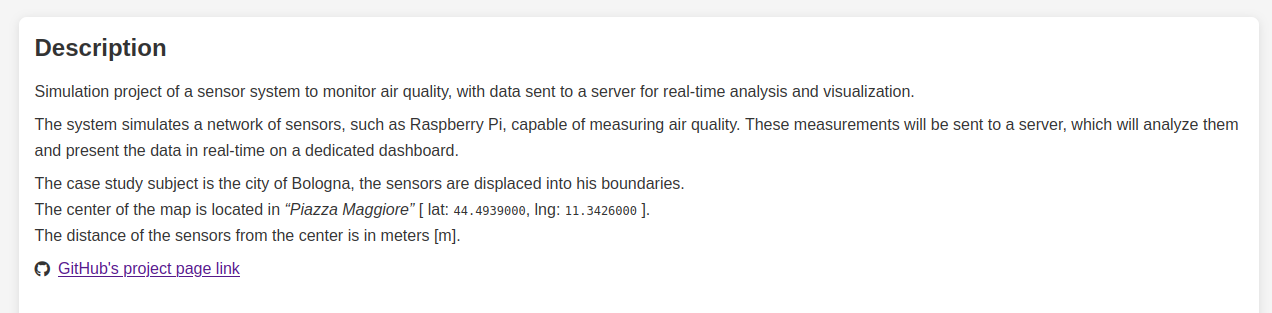
\includegraphics[width=\textwidth]{dashboard/00_disclaimer_description.png}
    \caption{Descrizione}
    \label{fig:app-description}
  \end{subfigure}

  \hfill
  \begin{subfigure}{\textwidth}
    \centering
    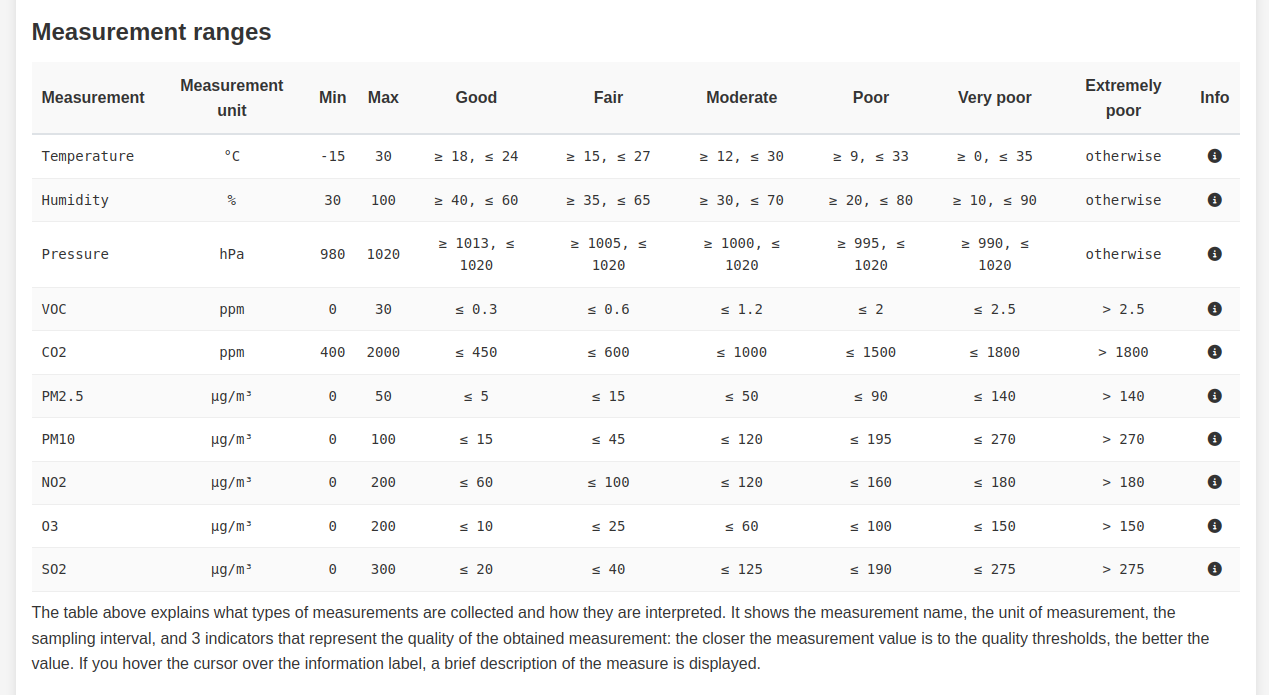
\includegraphics[width=\textwidth]{dashboard/01_table_measurement_ranges.png}
    \caption{Tabella valori riferimento \acrfull{eaqi}}
    \label{fig:app-eaqi-table}
  \end{subfigure}


  \hfill
  \begin{subfigure}{\textwidth}
    \centering
    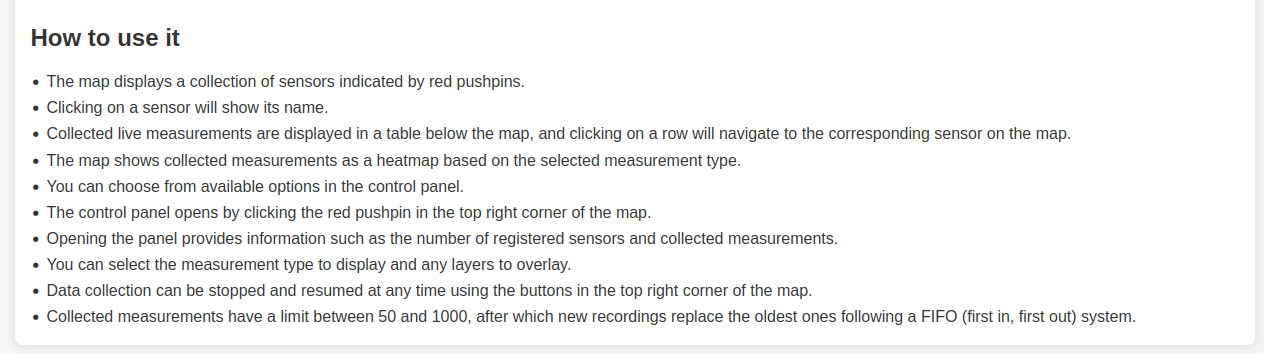
\includegraphics[width=\textwidth]{dashboard/02_disclaimer_how_to_use_it.png}
    \caption{Guida}
    \label{fig:app-guide}
  \end{subfigure}

  \hfill
  \begin{subfigure}{\textwidth}
    \centering
    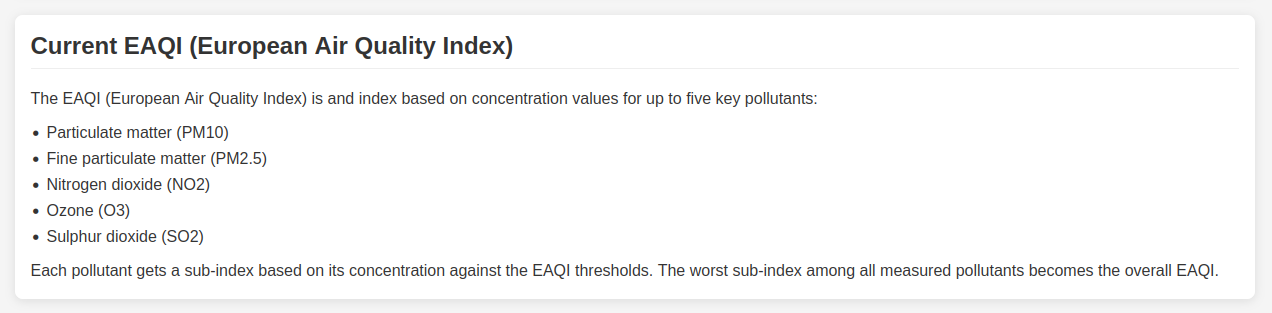
\includegraphics[width=\linewidth]{dashboard/03_disclaimer_eaqi.png}
    \caption{Calcolo \acrfull{eaqi}}
    \label{fig:app-eaqi-calculation}
  \end{subfigure}

  \caption{Intestazione web app}
  \label{fig:app-heading}
\end{figure}

\paragraph{Mappa}

Atterrando sulla pagina principale, viene presentata una mappa come da immagine \ref{fig:app-map-sensors}.
Tale mappa viene centrata su Bologna, e presenta i sensori registrati utilizzando degli spilli color rosso.
È possibile distinguere il centro della mappa, Piazza Maggiore, per via del colore blu del suo spillo,
come si può notare nell'immagine \ref{fig:app-map-center}.

\begin{figure}[H]
  \centering
  \begin{subfigure}{\textwidth}
    \centering
    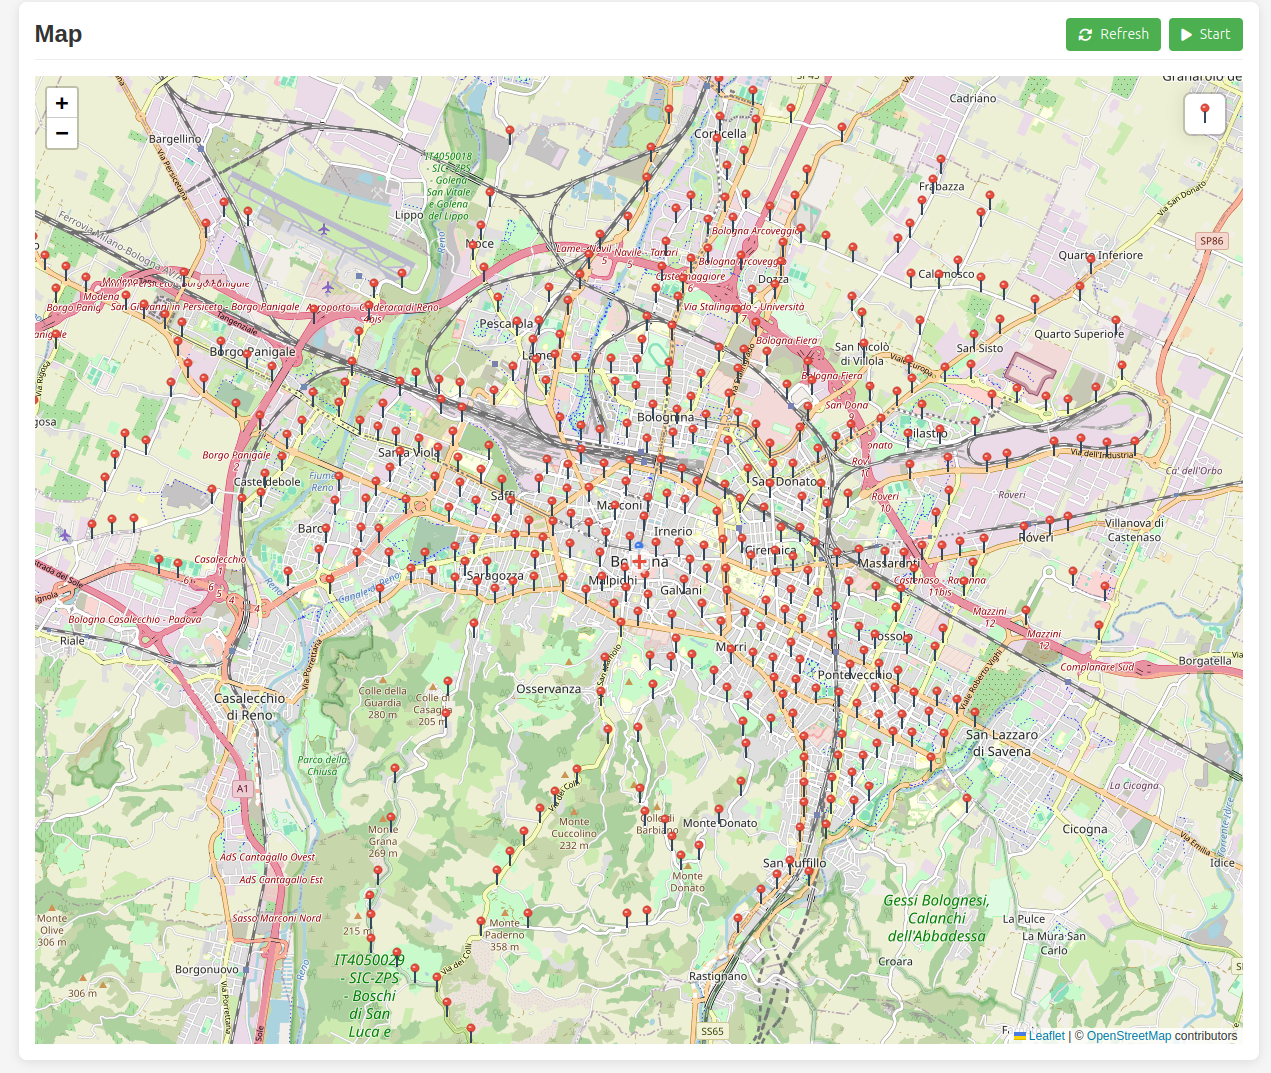
\includegraphics[width=\textwidth]{dashboard/04_map_sensors.png}
    \caption{Mappa principale}
    \label{fig:app-map-sensors}
  \end{subfigure}

  \hfill
  \begin{subfigure}{\textwidth}
    \centering
    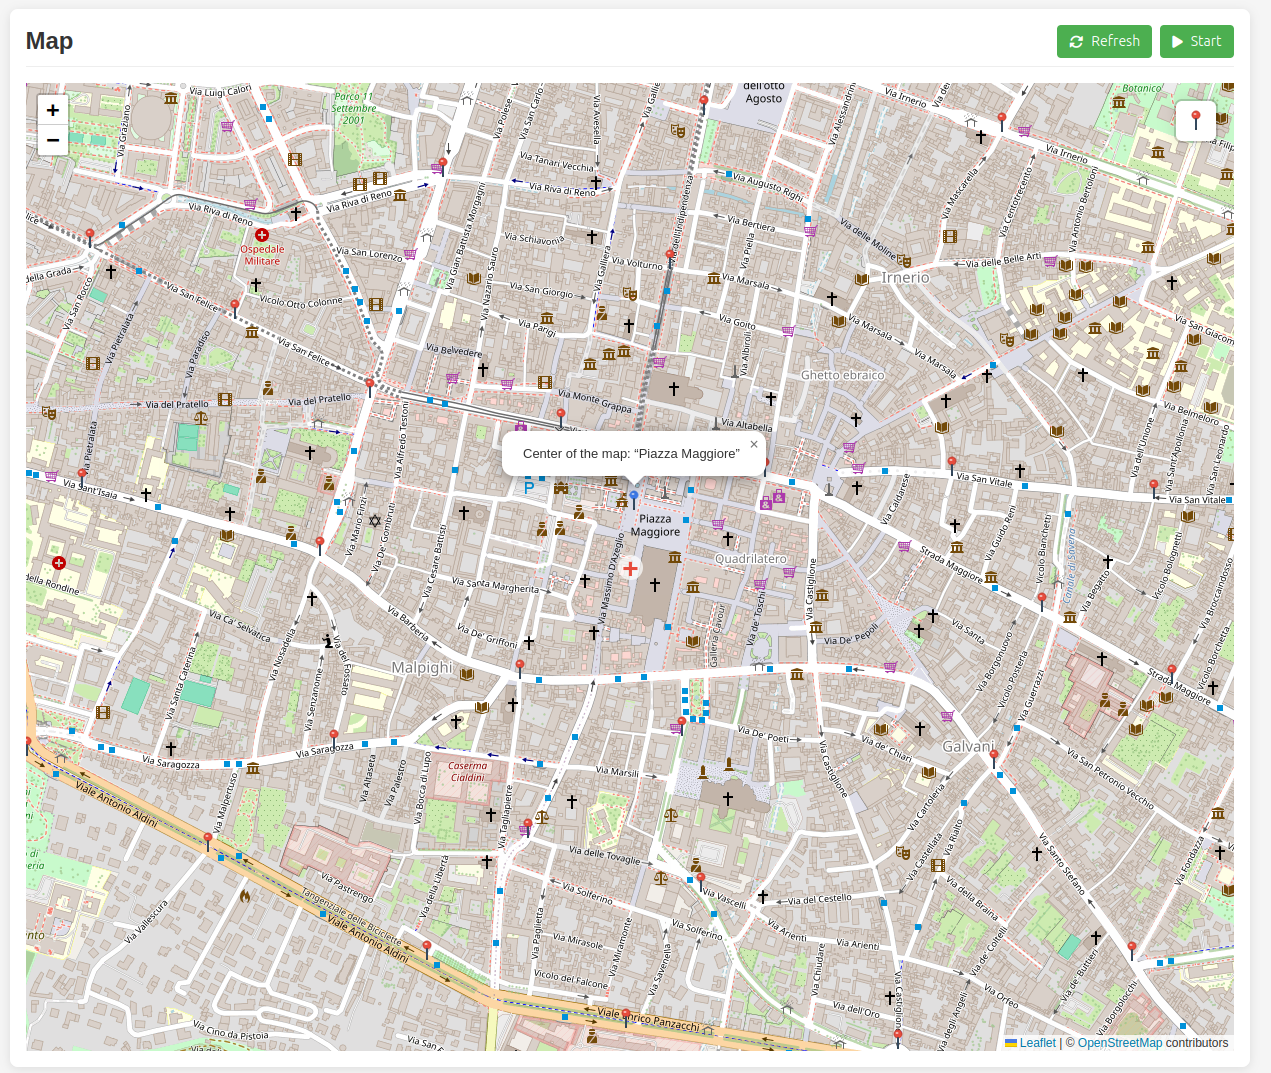
\includegraphics[width=\textwidth]{dashboard/05_map_sensors_center_of_the_map.png}
    \caption{Centro della mappa}
    \label{fig:app-map-center}
  \end{subfigure}
\end{figure}

La mappa dispone di un pannello di controllo presente in alto a destra.
Cliccandovici sopra, tale pannello si espande, mostrando le informazioni sulla mappa attualmente
visualizzata e fornendo degli strumenti per interagire con essa.

Come prima voce si ha il numero dei sensori attualmente presenti in mappa.
Tale conteggio è globale e considera tutti i sensori forniti, indipendentemente dall'attuale stato dei singoli,
che siano quindi attivi o meno. Lo stato è una proprietà booleana del sensore chiamata \texttt{status}
che esprime lo stato di "attivo" («\texttt{active}») se accesa.  Nelle tabella in figura
\ref{fig:app-tab-registered-sensors} è possibile vedere gi attributi dei sensori, precedentemente esposti nella lista
\ref{lst:sensors-properties}.

TODO Parlare di come si calcola la distanza dal centro!

\begin{figure}[H]
  \centering

  \begin{subfigure}{\textwidth}
    \centering
    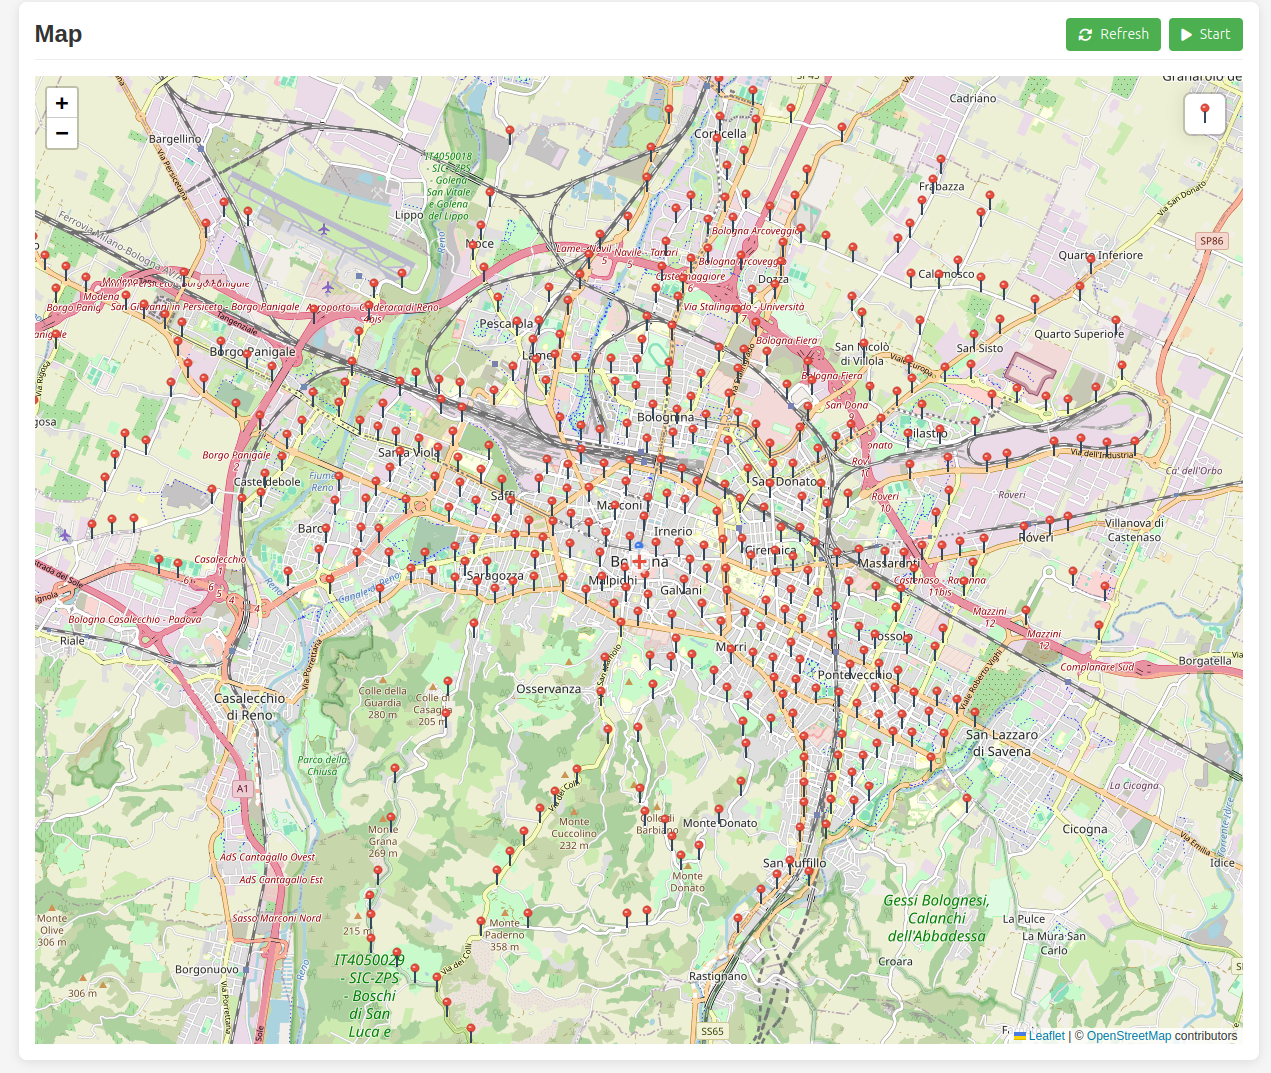
\includegraphics[width=\textwidth]{dashboard/04_map_sensors.png}
    \caption{Descrizione}
    % \label{fig:app-description}
  \end{subfigure}

\end{figure}

\paragraph{Heatmap}

Una heatmap (mappa di calore) è una rappresentazione grafica bidimensionale di dati in cui i valori individuali,
contenuti in una matrice, sono rappresentati attraverso colori \citep{wilkinson2009grammar}.
Questa tecnica di visualizzazione permette di identificare rapidamente pattern, correlazioni e anomalie
all'interno di dataset complessi mediante l'uso di una scala cromatica che associa intensità di colore
a valori numerici \citep{cleveland1993visualizing}. Il suo utilizzo aiuta a rendere più intuitiva la distribuzione
dei dati poiché a maggior concentrazione risulta un colore più intenso, facilitandone la comprensione ed attirando
l'attenzione sui principali focolai.

Formalmente, data una matrice $M \in \mathbb{R}^{m \times n}$ dove $M_{ij}$ rappresenta il valore
nella posizione $(i,j)$, una heatmap è una funzione di mappatura $ f: M_{ij} \rightarrow C_{ij} $
dove $C_{ij}$ è il colore corrispondente al valore $M_{ij}$ secondo una scala cromatica predefinita.

La scelta della palette di colori è cruciale per l'efficacia comunicativa della heatmap.
È fondamentale utilizzare scale cromatiche che rispettino principi di accessibilità e che siano percettivamente
uniformi \citep{ware2012information}.
Tali colori sono infatti quelli forniti dall'\acrfull{eea} come indicato nella tabella~\ref{tab:air_quality};

Nelle immagini seguenti viene mostrata la heatmap relativa alle misurazioni di \acrshort{pm25}.
Partendo dalla vista default in immagine \ref{fig:app-map-pm25-controls-15},
passiamo ad una versione con zoom inferiore senza sensori \ref{fig:app-map-pm25-controls-16} e
con sensori \ref{fig:app-map-pm25-controls-17}.
Successivamente diminuiamo ulteriormente lo zoom senza sensori \ref{fig:app-map-pm25-controls-18}, per poi
riavvicinarci \ref{fig:app-map-pm25-controls-19}, visualizzarle la ZTL \ref{fig:app-map-pm25-controls-20} ed i
quartieri\ref{fig:app-map-pm25-controls-21}.
Infine, visualizziamo una versione con concentrazioni più elevate \ref{fig:app-map-pm25-controls-22}
rispetto alle prime, essendo passato più tempo ed avendo quindi un numero maggiore di misurazioni, e le altre
misurazioni disponibili \ref{fig:app-map-pm25-controls-23}.

Come anticipato, allontanarci dal centro della mappa porterà a concentrazioni maggiori, mentre avvicinarci il contrario.
Anche il numero di misurazioni influisce sulle concentrazioni della mappa di calore, essendo direttamente correlate.
% L'utilizzo delle zone delimitate quali ZTL ed i quartieri può essere utile qualora si voglia verificare
% eventuali correlazioni fra le aree di maggiore concentrazione di inquinanti ed i confini amministrativi.

\begin{figure}[H]
  \centering
  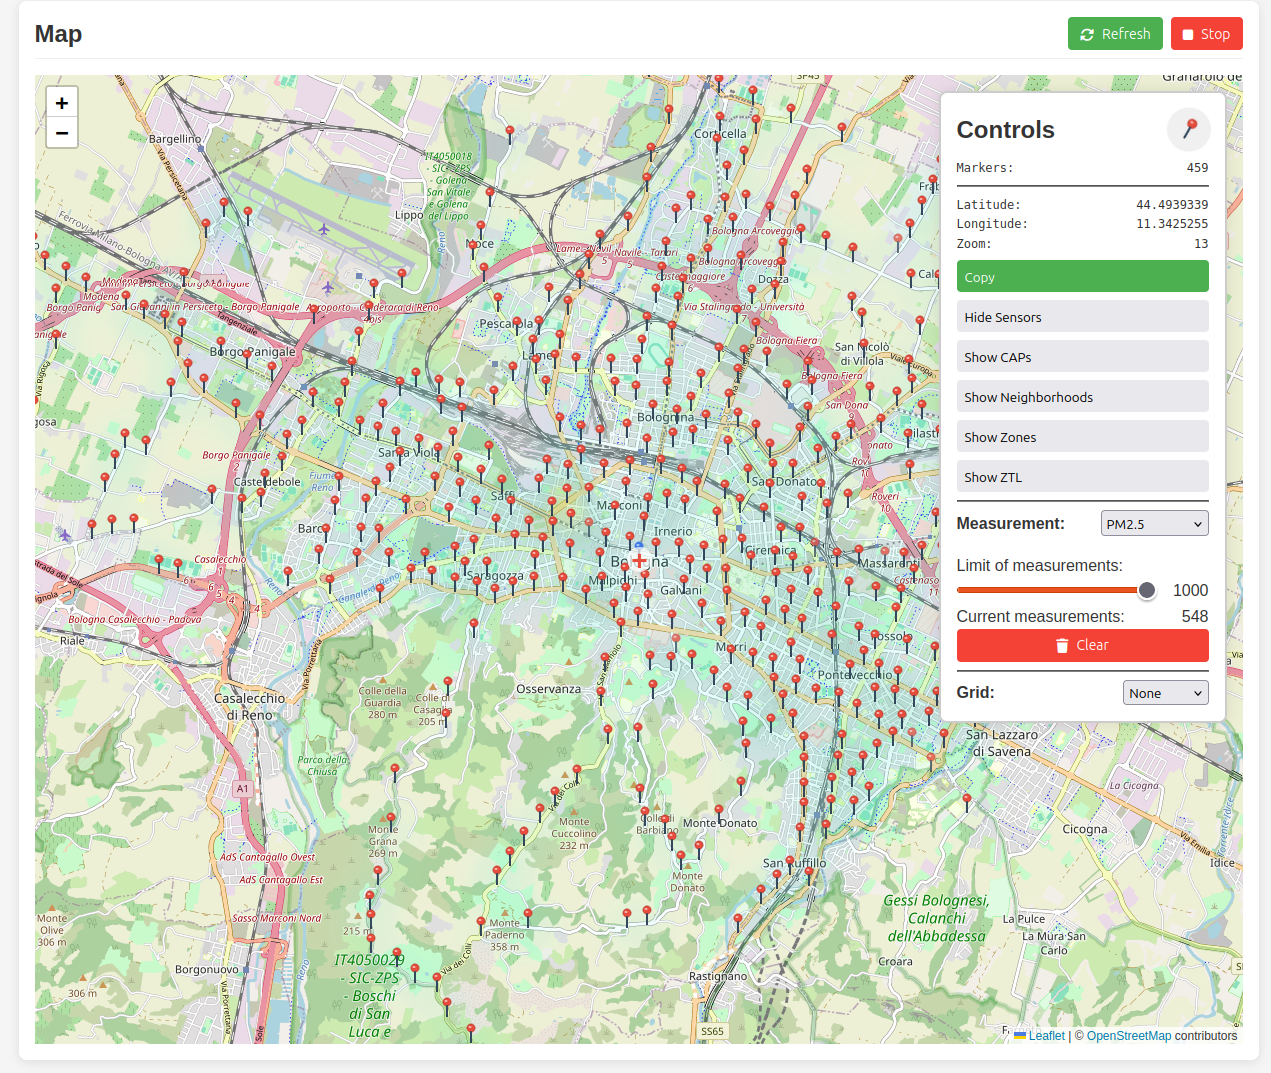
\includegraphics[width=0.95\textwidth]{dashboard/15_map_pm25_controls.png}
  \caption{Heatmap default}
  \label{fig:app-map-pm25-controls-15}

  \hfill

  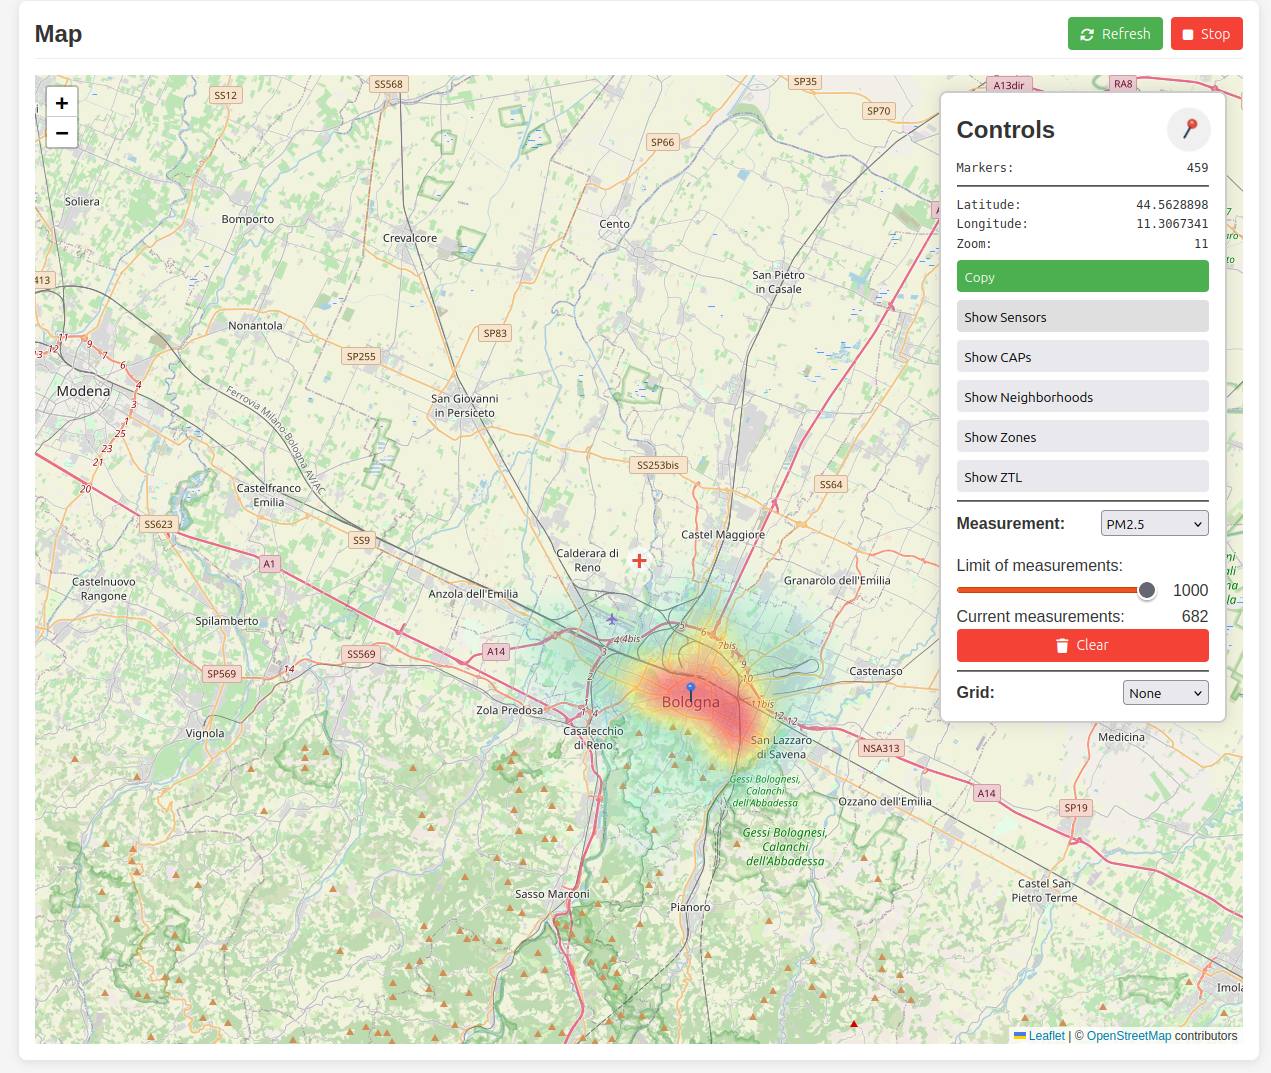
\includegraphics[width=0.95\textwidth]{dashboard/16_map_pm25_controls.png}
  \caption{Heatmap zoom 11 senza sensori}
  \label{fig:app-map-pm25-controls-16}
\end{figure}

\begin{figure}[H]
  \centering
  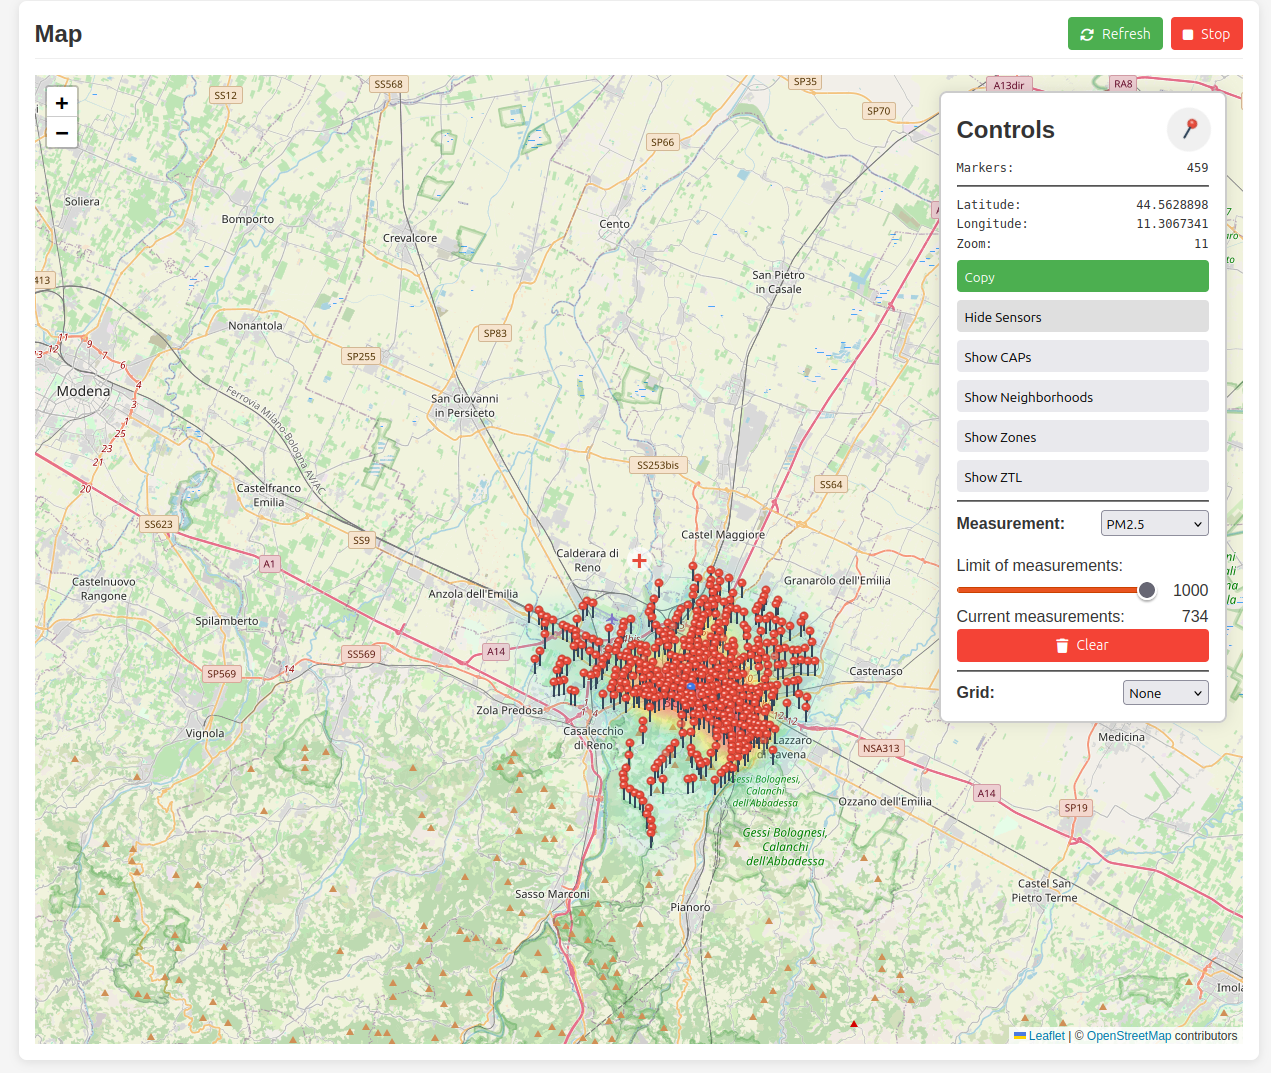
\includegraphics[width=0.95\textwidth]{dashboard/17_map_pm25_controls.png}
  \caption{Heatmap zoom 11 con sensori}
  \label{fig:app-map-pm25-controls-17}

  \hfill

  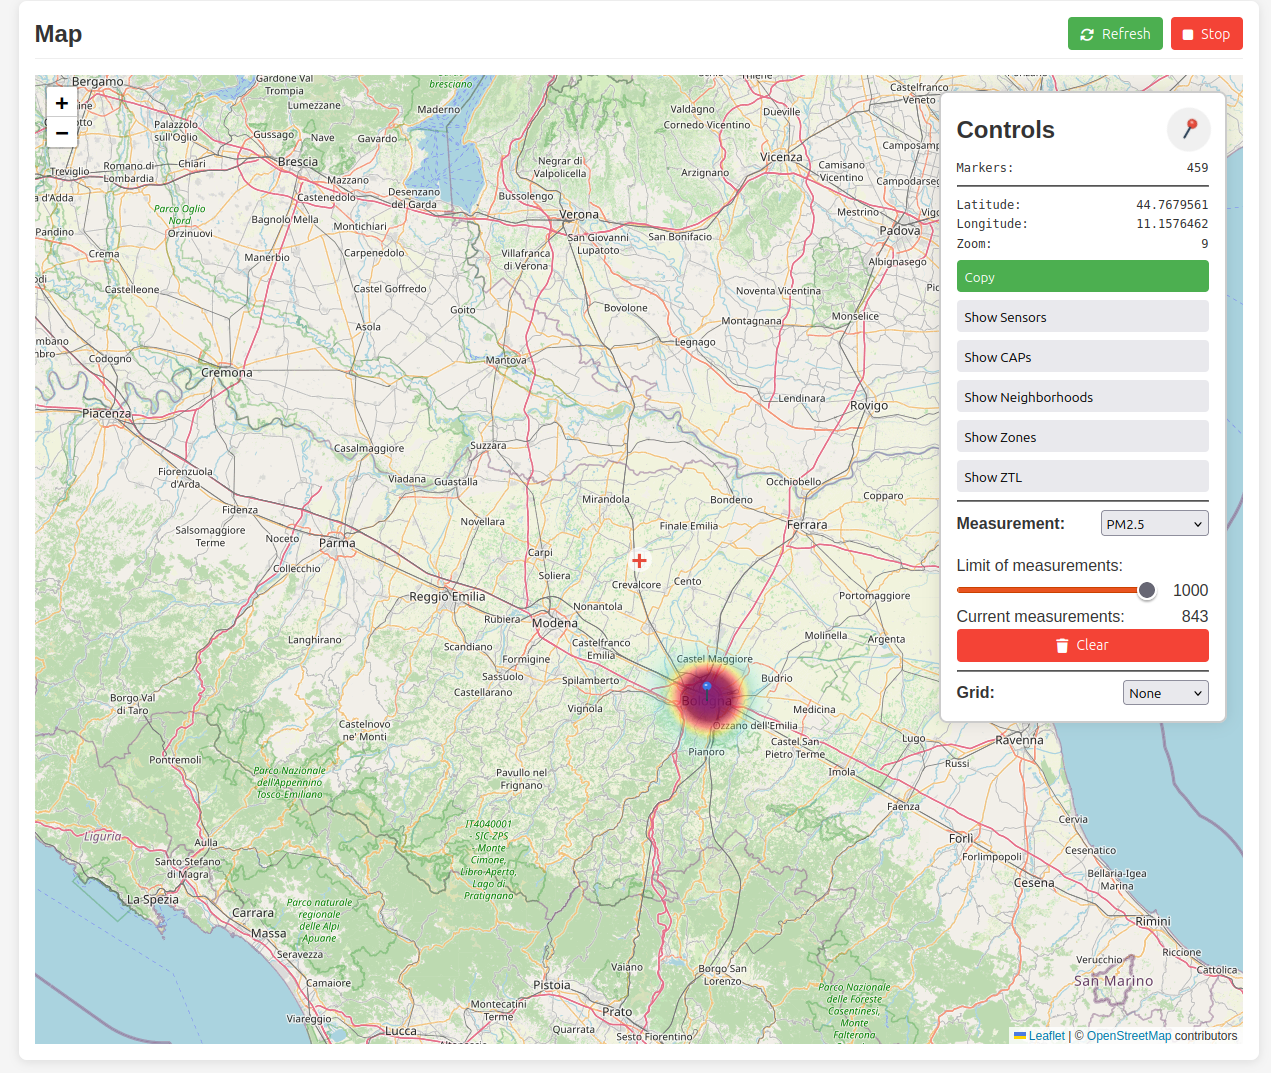
\includegraphics[width=0.95\textwidth]{dashboard/18_map_pm25_controls.png}
  \caption{Heatmap zoom 9 senza sensori}
  \label{fig:app-map-pm25-controls-18}
\end{figure}

\begin{figure}[H]
  \centering
  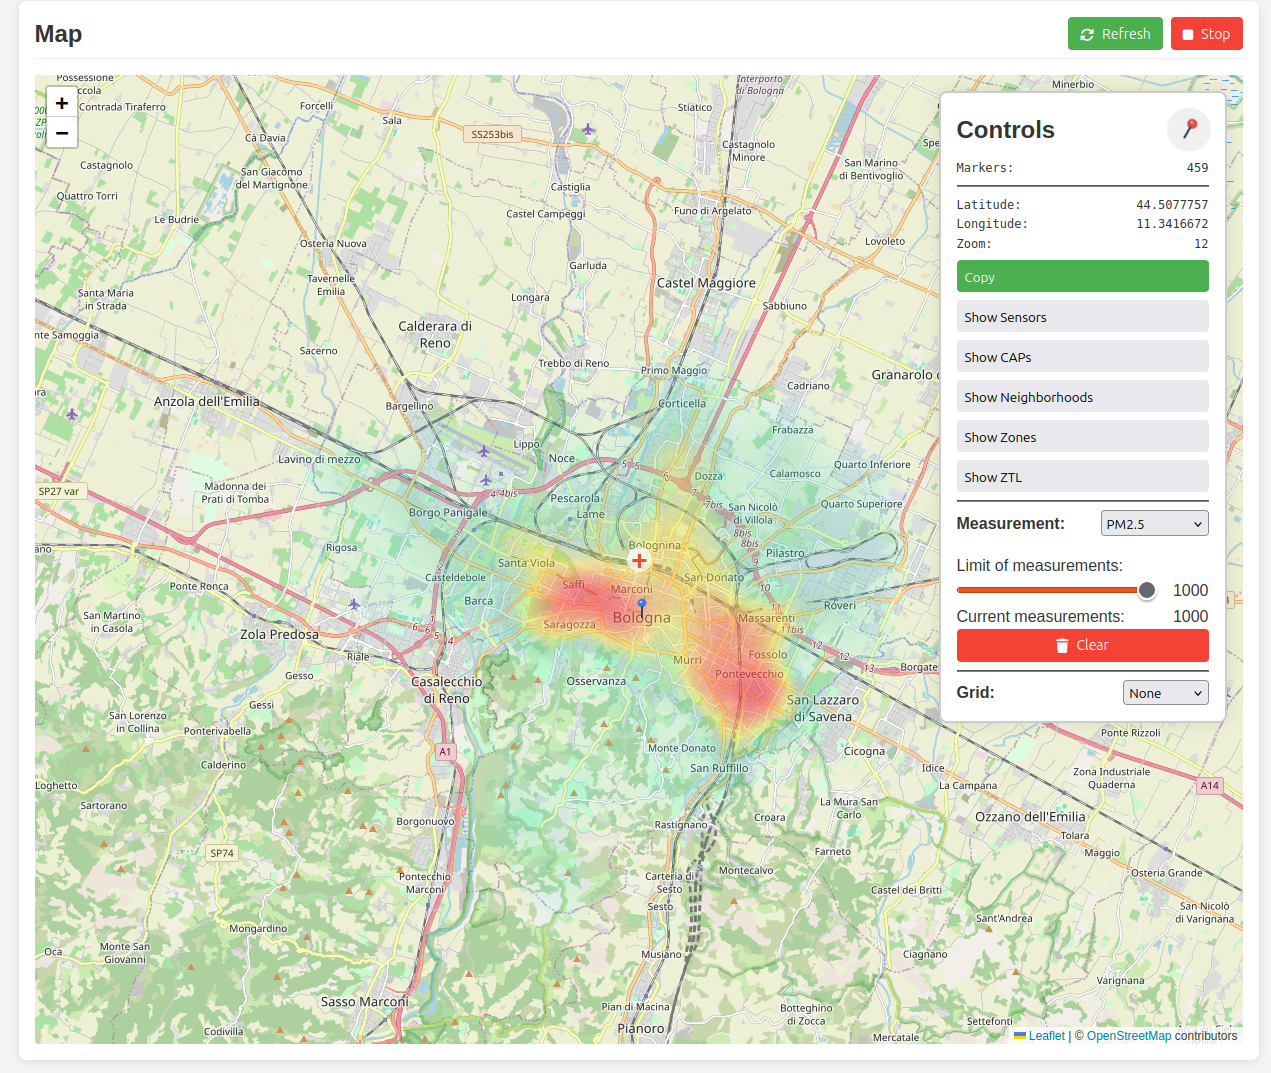
\includegraphics[width=0.95\textwidth]{dashboard/19_map_pm25_controls.png}
  \caption{Heatmap zoom 12 senza sensori}
  \label{fig:app-map-pm25-controls-19}

  \hfill

  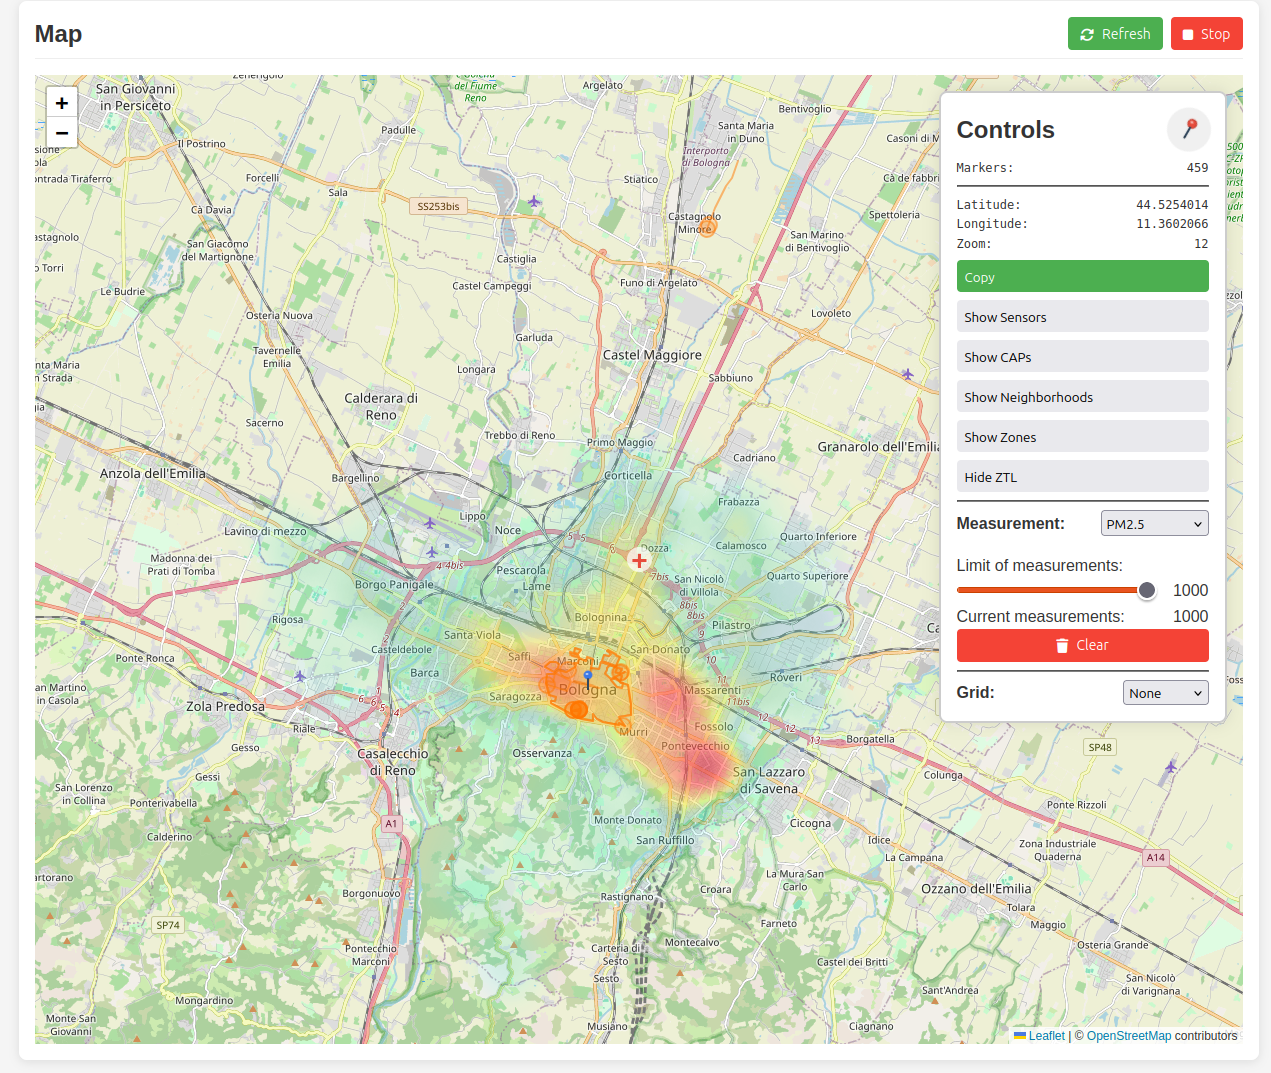
\includegraphics[width=0.95\textwidth]{dashboard/20_map_pm25_controls.png}
  \caption{Heatmap zoom 12 senza sensori con ZTL}
  \label{fig:app-map-pm25-controls-20}
\end{figure}

\begin{figure}[H]
  \centering
  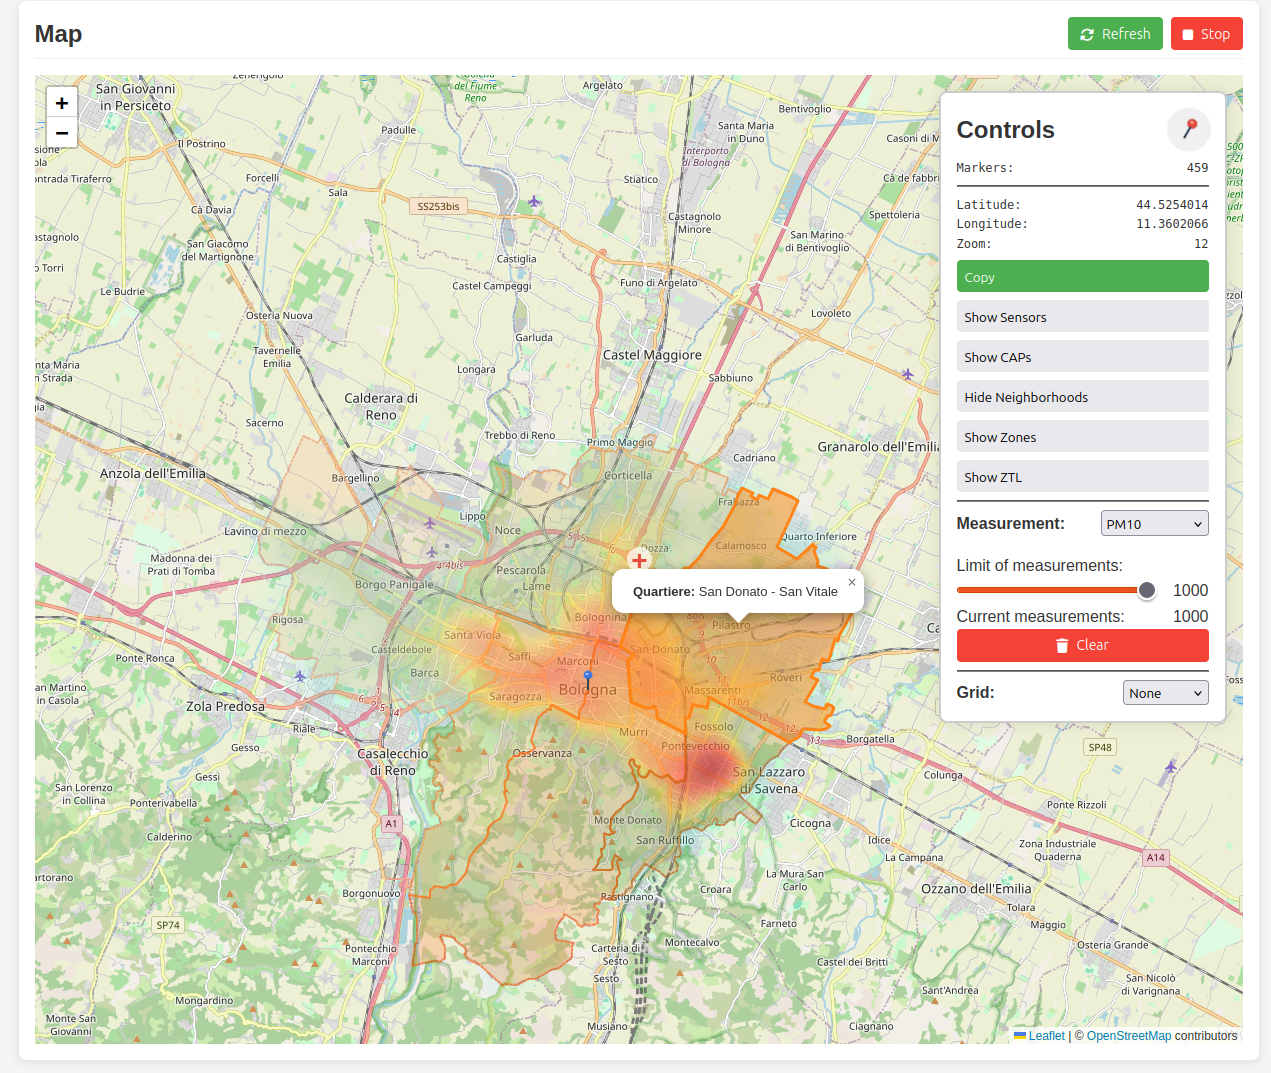
\includegraphics[width=0.95\textwidth]{dashboard/21_map_pm25_controls.png}
  \caption{Heatmap zoom 12 senza sensori con quartieri}
  \label{fig:app-map-pm25-controls-21}

  \hfill

  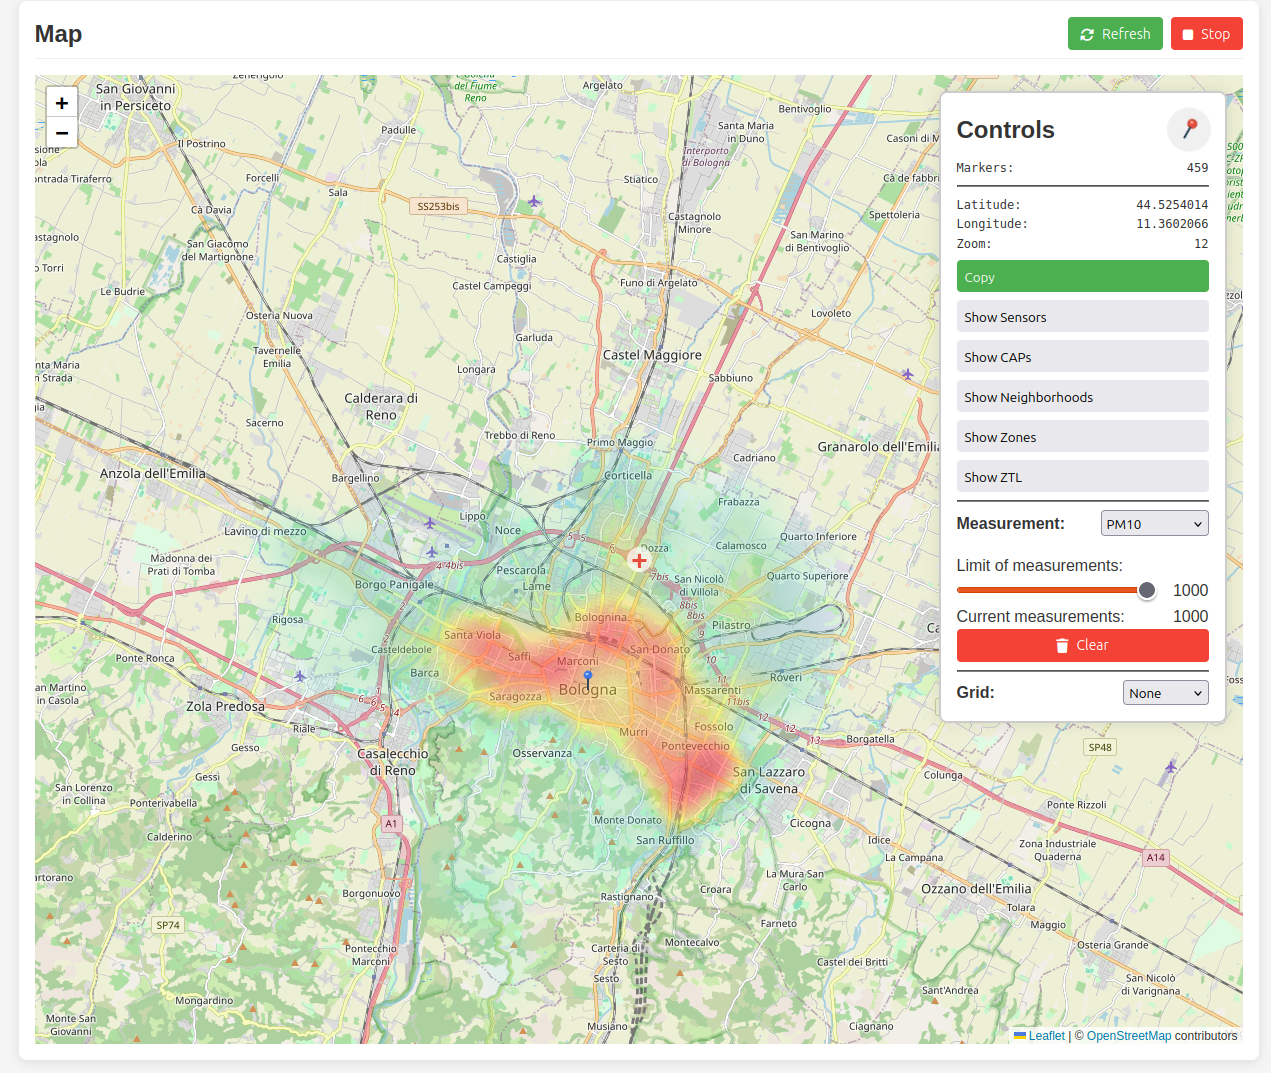
\includegraphics[width=0.95\textwidth]{dashboard/22_map_pm25_controls.png}
  \caption{Heatmap zoom 12 senza sensori, concentrazione maggiore}
  \label{fig:app-map-pm25-controls-22}
\end{figure}

\begin{figure}[H]
  \centering
  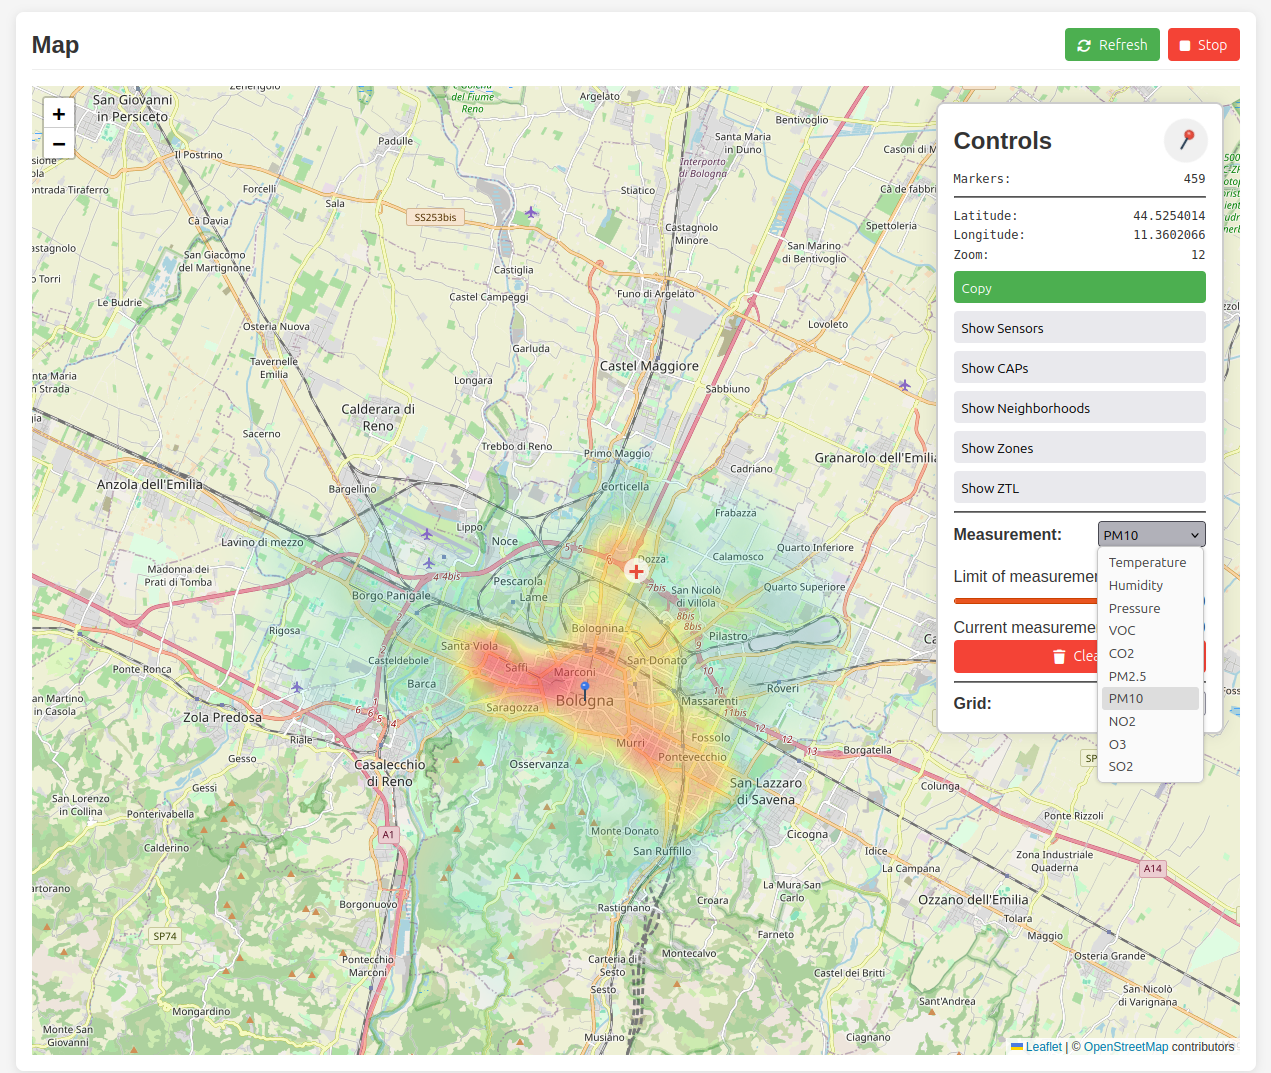
\includegraphics[width=0.95\textwidth]{dashboard/23_map_pm25_controls.png}
  \caption{Heatmap zoom 12 senza sensori, apertura lista misurazioni disponibili}
  \label{fig:app-map-pm25-controls-23}
\end{figure}

\paragraph{Ultime misuraizoni}

TODO

\begin{figure}[H]
  \centering
  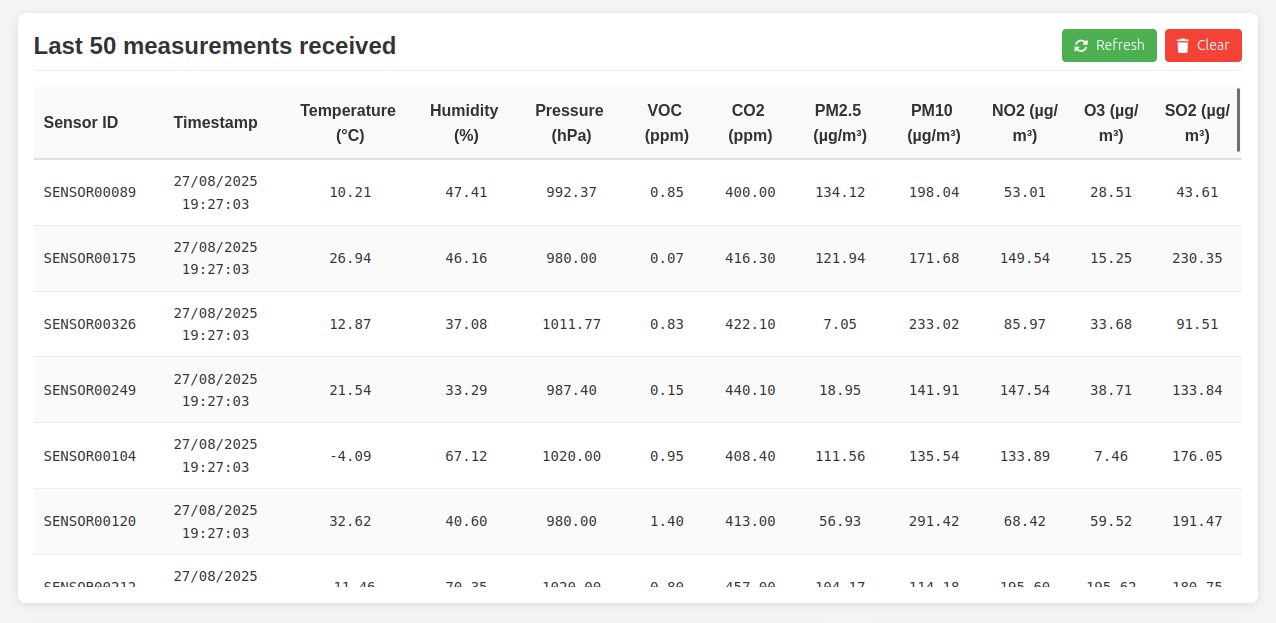
\includegraphics[width=\textwidth]{dashboard/24_table_last_measurements.png}
  \caption{Ultime misurazioni}
  \label{fig:app-tab-last-measurements}
\end{figure}
\paragraph{Statistiche}

TODO Statistiche

\begin{figure}[H]
  \centering
  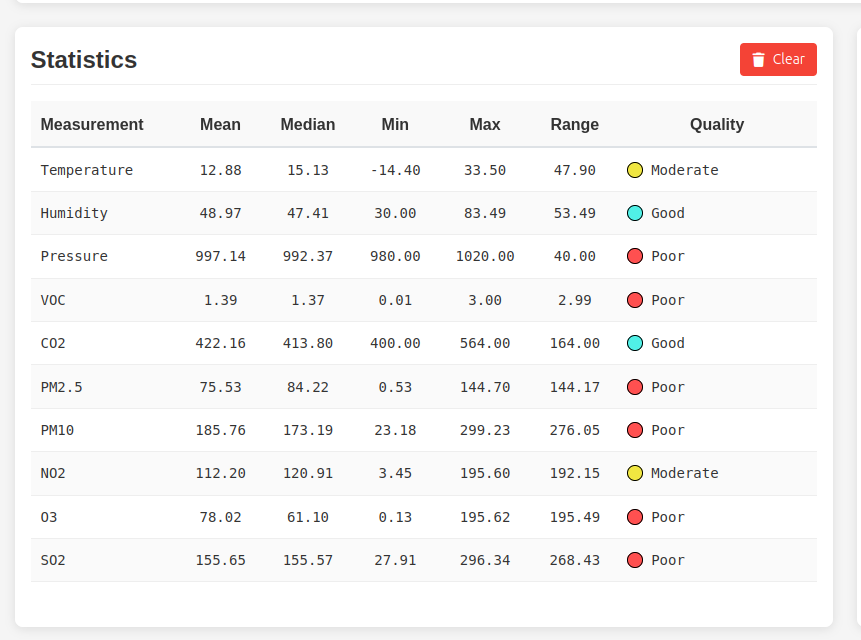
\includegraphics[width=\textwidth]{dashboard/25_table_statistics.png}
  \caption{Tabella statistiche}
  \label{fig:app-tab-statistics}
\end{figure}

\paragraph{Log di sistema}

Le interazioni con l'applicazioni, che siano da interfaccia utente o tramite \acrshort{api}, vengono elencate
nella tabella del log di sistema. Eventi quali la ricezione di una nuova misurazione, il cliccare

\begin{figure}[H]
  \centering
  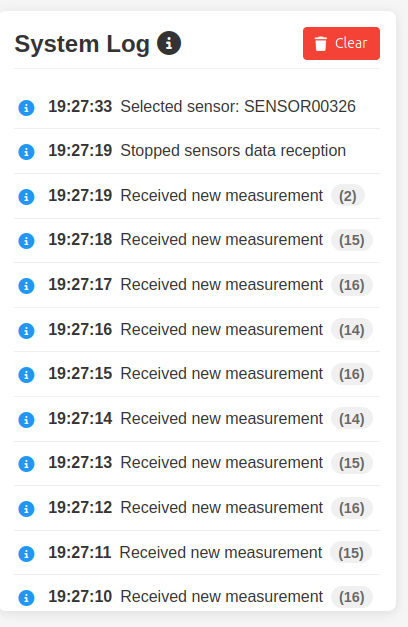
\includegraphics[width=\textwidth]{dashboard/26_table_system_log.png}
  \caption{Tabella log di sistema}
  \label{fig:app-tab-system-log}
\end{figure}

\paragraph{Tabella dei sensori registrati}

La parte finale della pagina principale riporta la tabella dei sensori registrati.

Questa tabella è formata da diverse colonne, quali l'id del sensore, latitudine, longitudine, stato,
distanza dal centro della mappa, data ultima misurazione registrata e relativo tempo trascorso da essa.

\begin{figure}[H]
  \centering
  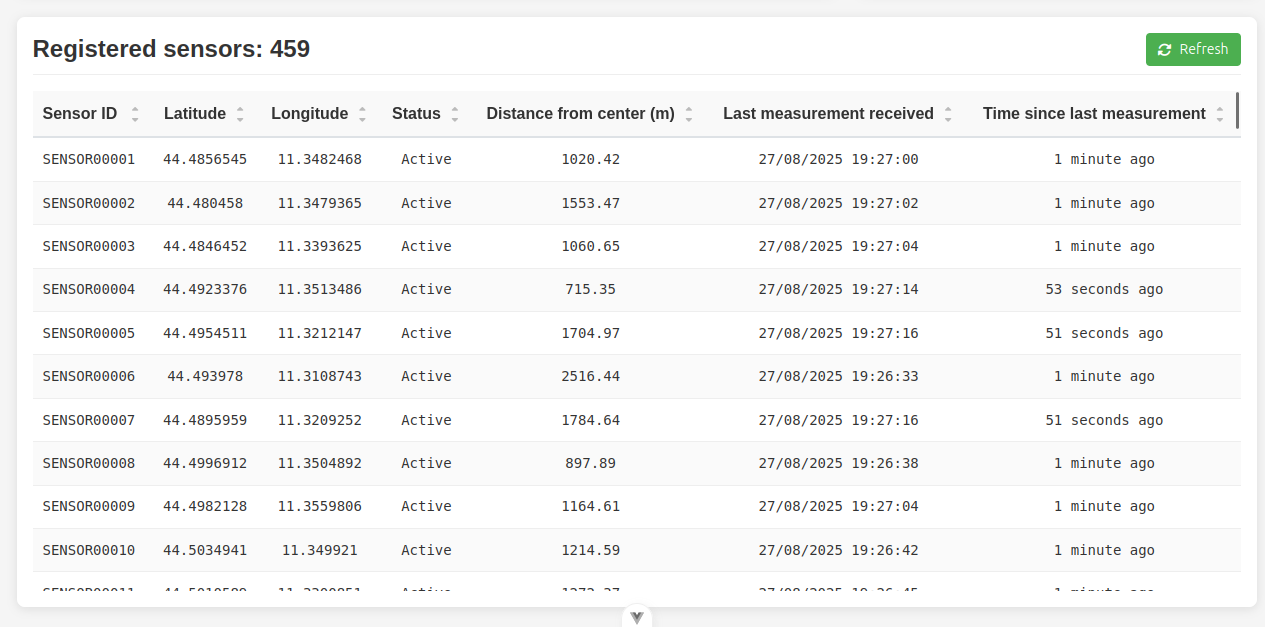
\includegraphics[width=\textwidth]{dashboard/27_table_registered_sensors.png}
  \caption{Tabella sensori registrati}
  \label{fig:app-tab-registered-sensors}
\end{figure}

Nella prima immagine~\ref{fig:app-tab-registered-sensors} abbiamo i sensori ordinati per id crescente (default),
mentre nella seconda~\ref{fig:app-tab-registered-sensors-distance-sort-asc} e
terza immagine~\ref{fig:app-tab-registered-sensors-distance-sort-desc} si ha la tabella ordinata rispetto
la distanza dal centro della mappa relativamente in ordine crescente (dal sensore più prossimo al più remoto) e
decrescente (dal sensore più lontano al più vicino).

\begin{figure}[H]
  \centering
  \begin{subfigure}{\textwidth}
    \centering
    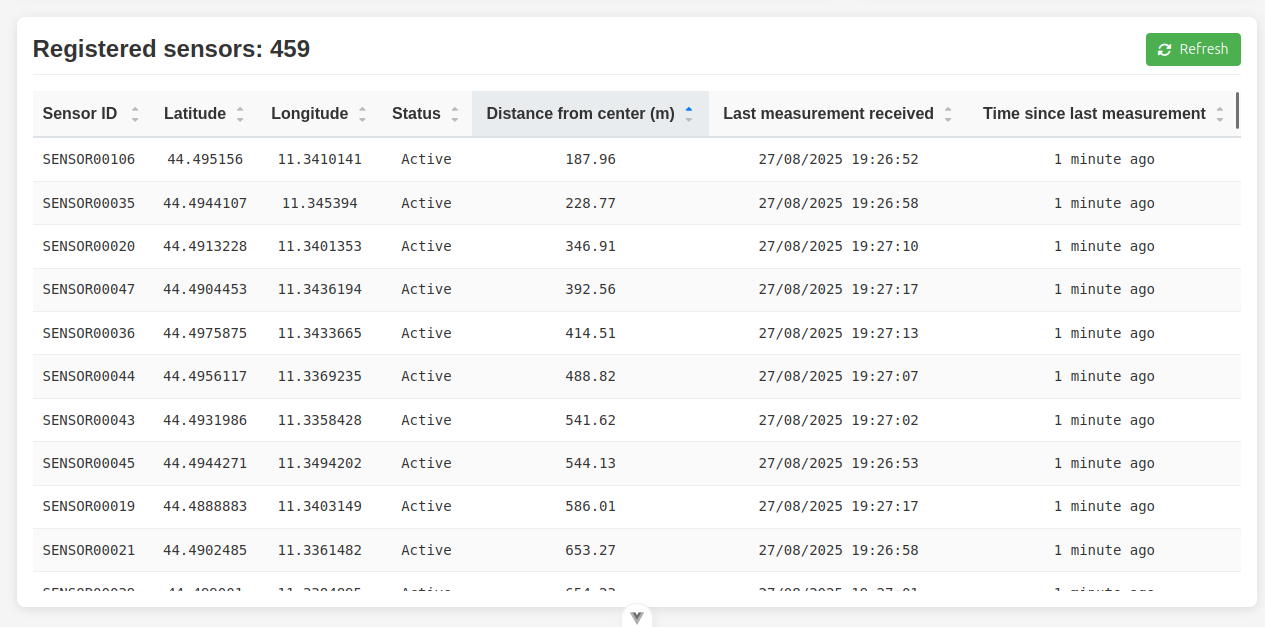
\includegraphics[width=\textwidth]{dashboard/28_table_registered_sensors_distance_sort_asc.png}
    \caption{Tabella sensori registrati, ordinati per "distanza dal centro" crescente}
    \label{fig:app-tab-registered-sensors-distance-sort-asc}
  \end{subfigure}

  \hfill
  \begin{subfigure}{\textwidth}
    \centering
    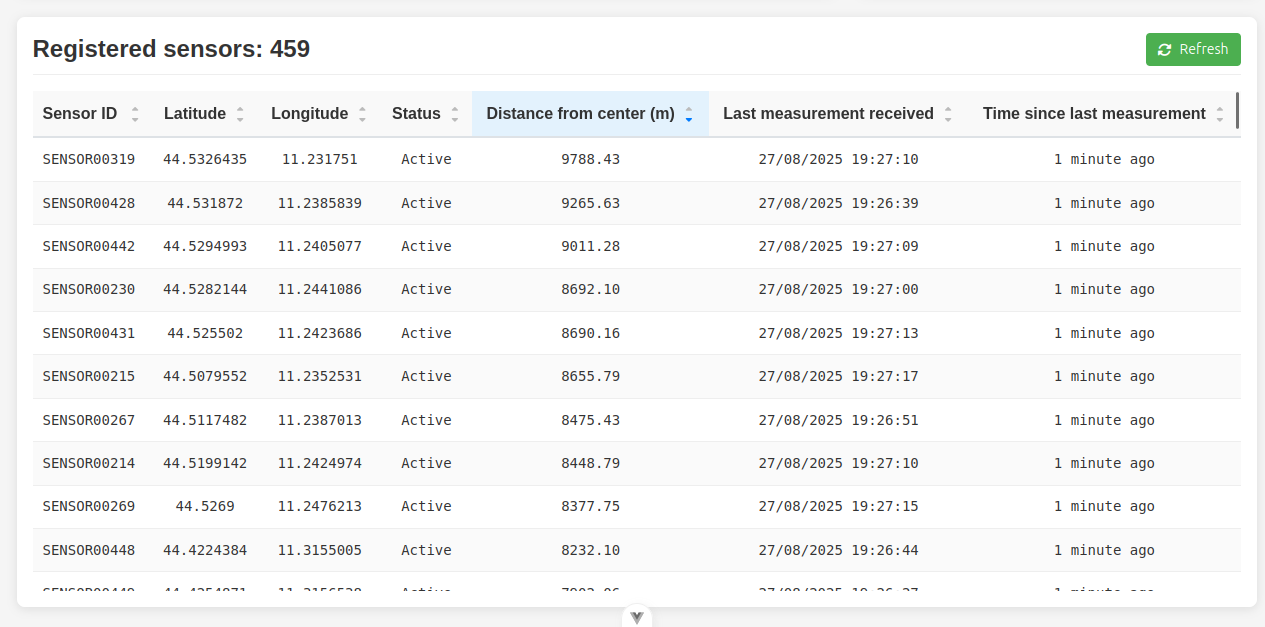
\includegraphics[width=\textwidth]{dashboard/29_table_registered_sensors_distance_sort_desc.png}
    \caption{Tabella sensori registrati, ordinati per "distanza dal centro" decrescente}
    \label{fig:app-tab-registered-sensors-distance-sort-desc}
  \end{subfigure}
\end{figure}

Il calcolo per tale distanza è realizzato attraverso la formula di Haversine \cite{haversine_formula},
ovvero una funzione usata per calcolare la distanza ortodromica (linea retta sulla superficie terrestre) tra due punti.
Essendo i sensori dotati di coordinate spaziali quali latitudine e longitudine, come il centro della mappa,
la formula è risultata l'ideale per calcolarne la distanza.

\paragraph{Formula di Haversine}

Di seguito la formula in termini matematici~\ref{lst:haversine-formula-math},
con relativa legenda~\ref{lst:haversine-formula-math-legend}, e la versione
di codice Javascript~\ref{lst:haversine-formula-code} realmente utilizzata dall'applicazione.

\begin{figure}[h]
  \begin{align}
    a & = \sin^2\left(\frac{\Delta\varphi}{2}\right) + \cos\varphi_1 \cdot \cos\varphi_2 \cdot \sin^2\left(\frac{\Delta\lambda}{2}\right) \\
    c & = 2 \cdot \text{atan2}\left(\sqrt{a}, \sqrt{1-a}\right)                                                                           \\
    d & = R \cdot c
  \end{align}
  \caption{Formula matematica di Haversine}
  \label{lst:haversine-formula-math}
\end{figure}

\begin{tabular}{ll}
  \textbf{Simbolo}       & \textbf{Significato}                                \\
  \hline
  $\varphi$              & latitudine (in radianti)                            \\
  $\varphi_1, \varphi_2$ & latitudine del punto 1 e punto 2                    \\
  $\Delta\varphi$        & differenza di latitudine ($\varphi_2 - \varphi_1$)  \\
  $\lambda$              & longitudine (in radianti)                           \\
  $\lambda_1, \lambda_2$ & longitudine del punto 1 e punto 2                   \\
  $\Delta\lambda$        & differenza di longitudine ($\lambda_2 - \lambda_1$) \\
  $R$                    & raggio terrestre medio (\~ 6371 km)                 \\
  $d$                    & distanza tra i punti (in metri o km)                \\
  $c$                    & distanza angolare (in radianti)                     \\
  $a$                    & termine intermedio                                  \\
  \label{lst:haversine-formula-math-legend}
\end{tabular}

\begin{lstlisting}[caption={Formual di Haversine in codice Javascript}, label=lst:haversine-formula-code]
  // Function to calculate the distance between two geographic points (Haversine formula)
  calculateDistance(lat1, lon1, lat2, lon2) {
    const R = 6371000; // Earth radius in meters
    const dLat = ((lat2 - lat1) * Math.PI) / 180;
    const dLon = ((lon2 - lon1) * Math.PI) / 180;
    const a =
      Math.sin(dLat / 2) * Math.sin(dLat / 2) +
      Math.cos((lat1 * Math.PI) / 180) *
      Math.cos((lat2 * Math.PI) / 180) *
      Math.sin(dLon / 2) *
      Math.sin(dLon / 2);
    const c = 2 * Math.atan2(Math.sqrt(a), Math.sqrt(1 - a));
    return R * c;
  }
\end{lstlisting}

\section{Database service}

\section{Applicazione front-end}